\begin{figure}
    \begin{center}
        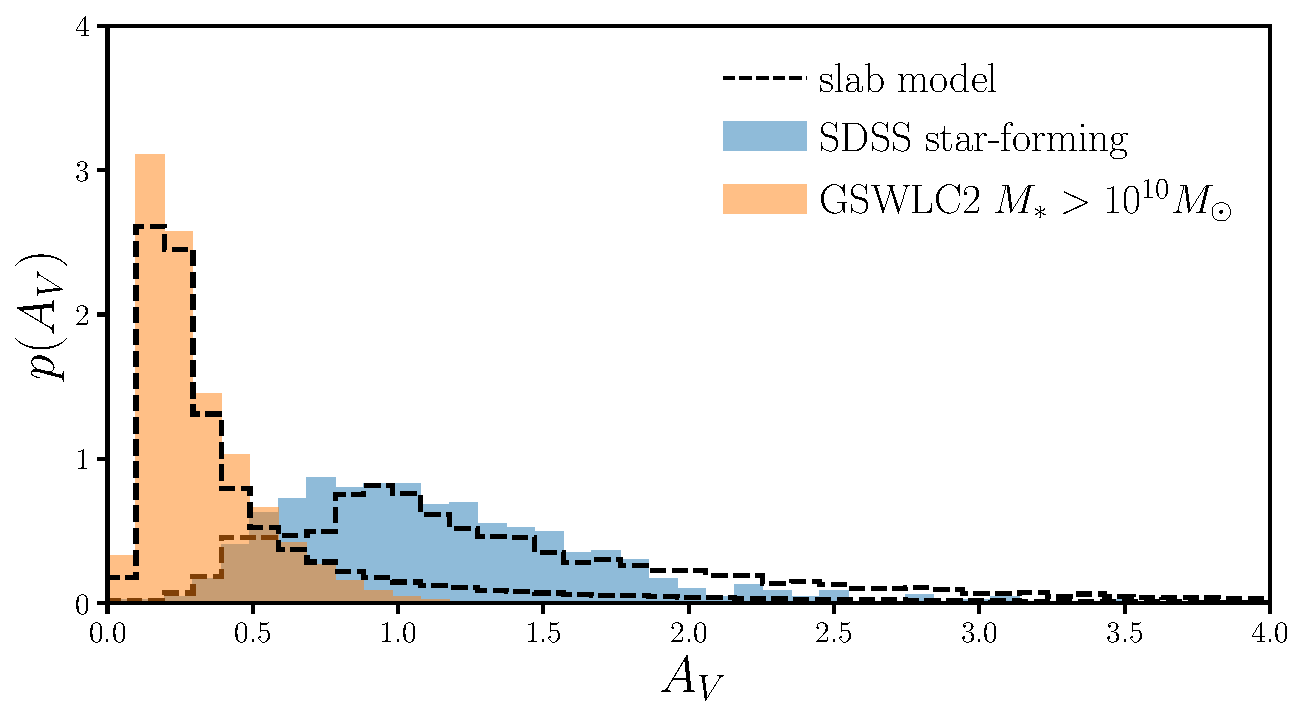
\includegraphics[width=0.66\textwidth]{figs/slab_model.pdf} 
        \caption{\label{fig:av_dist}
        The $A_V$ distributions, $p(A_V)$, generated from the slab model (Eq.~\ref{eq:slab};
        black dash) compared to $p(A_V)$ of star-forming galaxies in SDSS
        (blue) and of $M_* > 10^{10}M_\odot$ galaxies in the \cite{salim2018} GSWLC2 sample (orange). 
        The $A_V$ values for both observations are derived using SED
        fitting~\citep{brinchmann2004, salim2018}. 
        Meanwhile, for the slab model, we generate $A_V$ values for each galaxy
        in the SDSS and GSWLC2 samples using Eq.~\ref{eq:slab} with its
        measured $M_*$ and $\ssfr$. 
        The significant difference between the $p(A_V)$ of SDSS and GSWLC2 is
        due to inconsistencies in the $A_V$ measurements of the two catalogs. 
        It illustrates the challenges in observationally measuring $A_V$ and,
        again, highlights the advantages of our forward modeling approach. 
        Despite the significant differences between the two, the slab model is
        able to generate $p(A_V)$ in good agreement with $p(A_V)$ from both
        observations with parameter values chosen within the
        Table~\ref{tab:free_param} prior range. 
        Therefore, the slab model provides a sufficiently flexible prescription
        for our \eda.
        }
    \end{center}
\end{figure}


\section{The Slab Model Based EDA}  \label{sec:slab} 
\ch{ 
    In our \eda~prescription, we use the slab model to determine $A_V$, the
    amplitude of attenuation, as a function of a randomly sampled inclination,
    $i$, and $\tau_V$ (see Eq.~\ref{eq:slab} in Section~\ref{sec:dem}).
    The slab model is based on the assumption that dust in galaxies have
    slab-like geometry and illuminated by the stellar radiation
    source~\citep{somerville1999}. 
}
For a given $\tau_V$, the attenuation depends solely on the orientation of the galaxy. 
\ch{
    While this simplification reproduces the correlation between $A_V$ and $i$
    found in observed star-forming galaxies~\citep[\eg][]{conroy2010, wild2011,
    battisti2017, salim2020}, it ignores the detailed star-to-dust geometry that
    impacts the attenuation curve. 
    It also does not provide a well-motivated prescription for quiescent
    galaxies, which typically have elliptical morphologies.
    Despite its limitations, the slab model provides a robust empirical
    prescription that allows us to produce realistic distributions of $A_V$. 
}

\ch{ 
    In Figure~\ref{fig:av_dist}, we compare the $A_V$ distributions, $p(A_V)$,
    of star-forming galaxies in SDSS (blue) and galaxies in the
    \cite{salim2018} GSWLC2 sample (orange) to the $p(A_V)$ generated from the
    slab model (black dashed). 
    The $A_V$ values of the SDSS are derived using SED fitting from the
    \cite{brinchmann2004} MPA-JHU catalog.
    The $A_V$ values of the GSWLC2 galaxies are also derived from SED fitting UV and optical
    photometry from GALEX and SDSS observations as well as mid-IR photometry from WISE. 
    We include all GSWLC2 galaxies, including quiescent galaxies, above $M_* > 10^{10}M_\odot$. 
    We generate two $p(A_V)$ with the slab model for the SDSS and GSWLC2
    samples separately.
    For each SDSS/GSWLC2 galaxy, we determine $A_V$ by uniformly sampling 
    $\cos i$ from 0 to 1 and derive $\tau_V$ (Eq.~\ref{eq:tauv}) with the
    galaxy's measured $M_*$ and $\ssfr$. 
    We pick $\mtaum, \mtaus, c_\tau$ values within the prior range
    (Table~\ref{tab:free_param}) by hand to roughly reproduce the SDSS and GSWLC2 $p(A_V)$
    distributions. 
}

\ch{
    Galaxies in SDSS and GSWLC2 have substantially different $p(A_V)$. 
    This is due to inconsistencies in the $A_V$ measurements of MPA-JHU and
    GSWLC2 --- even for the same galaxy, the $A_V$ measurements from the two
    catalogs differ significantly.
    This difference in $p(A_V)$ illustrates the challenges in directly measuring
    dust attenuation and yet again highlights the advantages of our forward
    modeling approach. 
    Despite the dramatic differences between the two, the slab model can
    produce $p(A_V)$ in good agreement with both observed distributions. 
    We therefore conclude that the slab model provides a sufficiently flexible
    prescription to sample a realistic distribution of $A_V$. 
}


\ch{
    In addition to the slab model, in the \eda, we also use a linear
    dependence on $M_*$ and $\ssfr$ in the $V$ band optical depth,
    $\tau_V$ (see Eq.~\ref{eq:tauv}).
    This parameterization is motivated by observations that find significant
    correlation between $A_V$ and $M_*$ and $\ssfr$~\citep[\eg~][]{garn2010, battisti2016, salim2020}. 
    We take a closer look at this correlation using the GWSLC2 sample in
    Figure~\ref{fig:dep}.
    We present the dependence of $A_V$ on $M_*$ (left panel) and $\ssfr$ (right
    panel). 
    In the left panel, we divide the GSWLC2 galaxies by $\ssfr$: 
    $\ssfr < 10^{-11}yr^{-1}$ (purple), $10^{-11} < \ssfr < 10^{-10}yr^{-1}$
    (red), and  $10^{-10} < \ssfr$ (orange). 
    For each of the $\ssfr$ bins, we find significant $\log M_*$ dependence in
    $A_V$: galaxies with higher $\ssfr$ have a stronger $M_*$ dependence.  
    In the right, we divide the galaxies by $M_*$: 
    $10^{9.5} < M_* < 10^{10.5}M_\odot$ (blue) and $10^{10.5} M_\odot < M_*$
    (green).
    Although both $M_*$ bins have some $\ssfr$ dependence, the dependence is
    stronger for galaxies with $M_* > 10^{10.5}M_\odot$. 
    This stellar mass limit roughly corresponds to galaxies that are included
    in our forward model (see Figure~\ref{fig:avmsfr}). 
    The $M_*$ and $\ssfr$ dependence we find in $A_V$ from the GSWLC2 sample is
    consistent with previous observations and further motivates our
    \eda~prescription.
}

\begin{figure}
\begin{center}
    %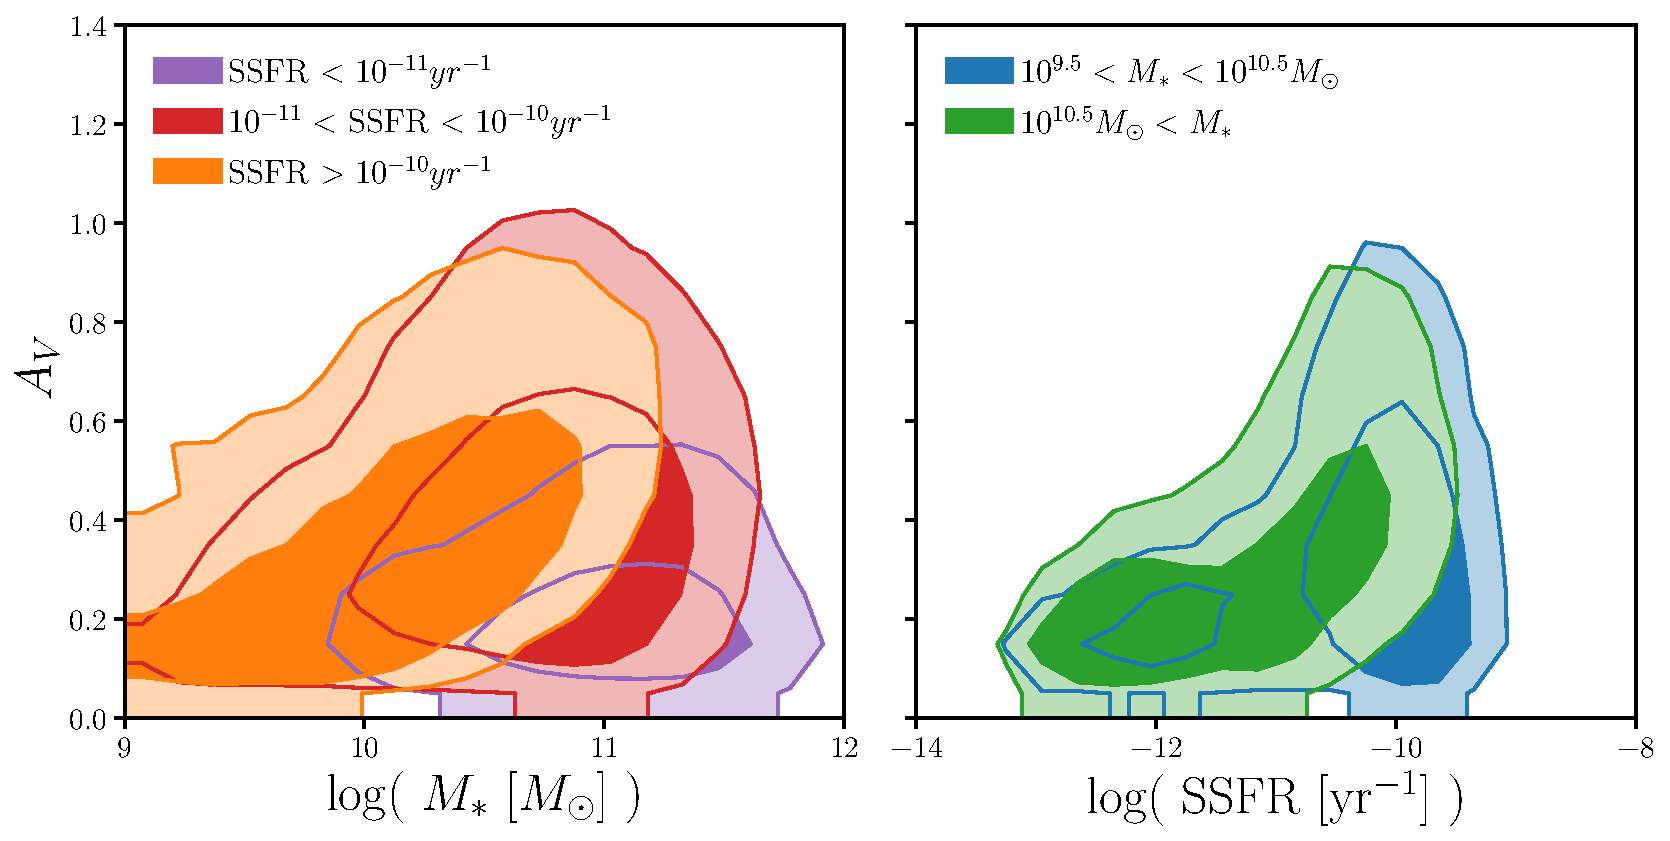
\includegraphics[width=\textwidth]{figs/gswlc_dep.pdf}
    \caption{\label{fig:dep}
    \ch{
        Dependence of $A_V$ on $M_*$ (left) and $\ssfr$ (right) for the
        \cite{salim2018} GSWLC2 sample.
        In the left panel, we divide the GSWLC2 sample into bins of $\ssfr$: 
        $\ssfr < 10^{-11}yr^{-1}$ (purple), 
        $10^{-11} < \ssfr < 10^{-10}yr^{-1}$ (red),
        and  $10^{-10} < \ssfr$ (orange). 
        In each of the $\ssfr$ bins, we find significant $M_*$ dependence. 
        In the right panel, we divide the sample into bins of $M_*$:  
        $10^{9.5} < M_* < 10^{10.5}M_\odot$ (blue) and $10^{10.5} M_\odot < M_*$ (green).
        In the $M_* > 10^{10.5}M_\odot$ bin, which roughly corresponds to our
        SDSS sample, we find significant $\ssfr$ dependence.
        The $M_*$ and $\ssfr$ dependence in $A_V$ we find in GSWLC2 is
        consistent with previous works and provides further motivation for our
        \eda~prescription.
    }
    }
\end{center}
\end{figure}
